\subsection{Empfehlung}

\subsubsection{Optimierungen}

\textbf{Antriebskonzept der Vereinzelung}
\newline
Die Inbetriebnahme der Vereinzelung zeigte, dass diese Funktion zuverlässig funktioniert. Dabei wurde auch erkannt, dass ohne Abstreifer erhebliches Spiel an der Lochmaske auftritt. Das Auftreten des Fehlers lässt sich durch zwei Gründe erklären
\begin{itemize}
	\item Das Funktionsmuster wurde ohne Motor realisiert. Durch das manuelle Testen von Hand, war Spiel nicht existent.
	
	\item Die hohe Übersetzung des Getriebemotors führt zu einem hohen Spiel an der Welle. Dieser Einfluss wurde in diesem Ausmass unterschätzt.
\end{itemize}

Zur Eliminierung des Spiels werden folgende Massnahmen empfohlen:

\begin{itemize}
	\item Der qualitativ durchschnittliche Antrieb (Pololu XY) durch einen qualitativ besseren Motor ersetzen, welcher ein geringeres Spiel aufweist.
	
	\item Die Anordnung des Antriebs neu konzipieren. Dabei kann das Spiel massiv reduziert werden, indem der Antrieb an der Aussenkontur der Lochmaske gekoppelt wird. Dabei muss an der Aussenkontur eine Verzahnung realisiert werden, sodass über ein zweites Zahnrad der Motor die Rotation umsetzen kann (siehe Abbildung \ref{fig:optimierung_lochmaske}). Die Grössenordnung dieser Übersetzung ist variabel, führt jedoch bei optimaler Auslegung dazu, dass ein Antrieb mit geringerer Übersetzung verwendet werden kann. Dadurch wird das Spiel reduziert. 
\end{itemize}
Dabei ist anzumerken, dass es sich hier um eine optionale Massnahme handelt. Die Funktion der Vereinzelung ist zum jetzigen Zeitpunkt zufriedenstellend.
\begin{figure}[H]
	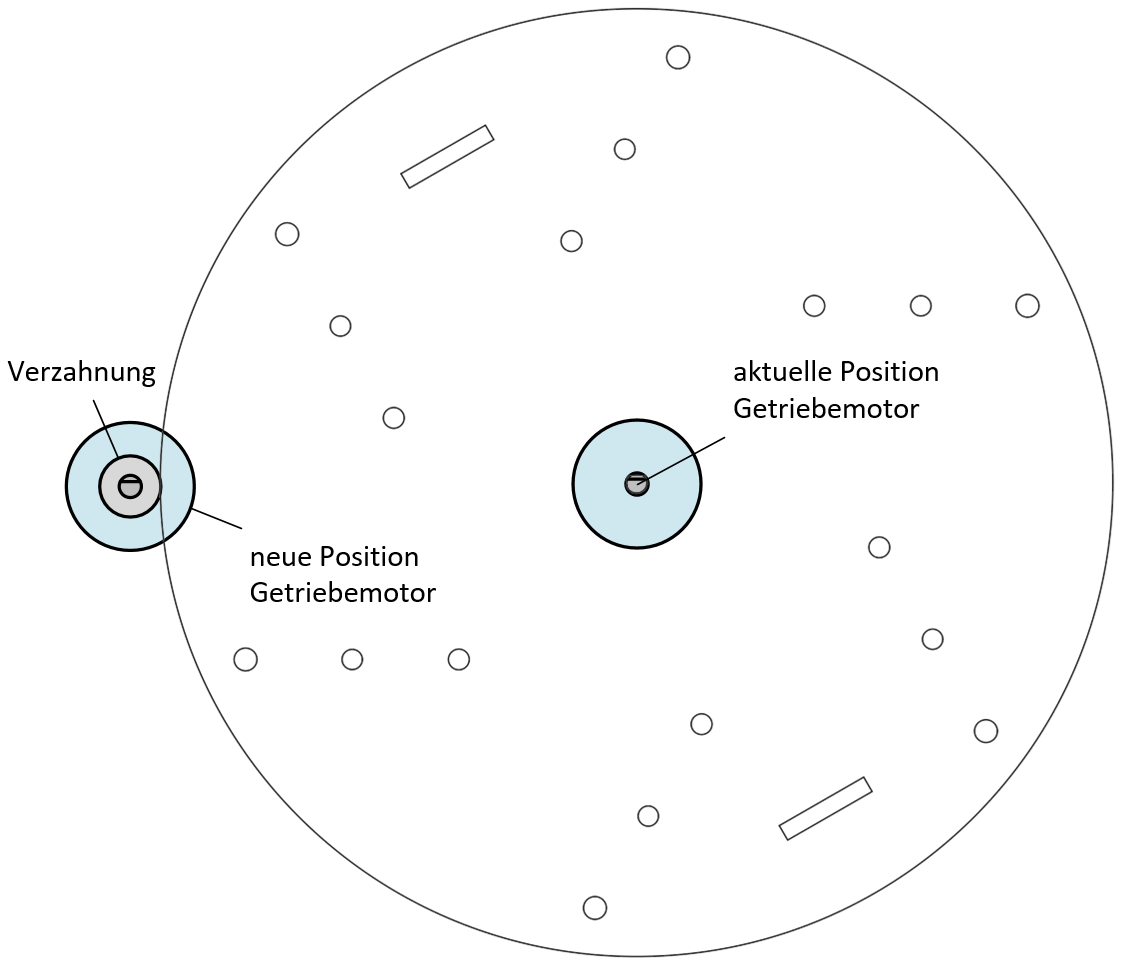
\includegraphics[scale=0.5]{Illustrationen/8-Fazit/optimierung_lochmaske.png}
	\caption{verbesserte Anordnung des Antriebs für die Lochmaske}
	\label{fig:optimierung_lochmaske}
\end{figure}